\chapter{Design Space Exploration for Implementation of Proposed Mechanisms}
\label{sec:design_space_exploration}

In this chapter, we consider multiple design choices for implementing the mechanisms proposed in this dissertation. The aim of the design space exploration is to come up with the best design for each mechanism in the context of operation in a geo-distributed setting. The chosen design should be scalable with respect to the number of clients and Edge sites, should perform the desired functionality expected from the mechanism effectively and not result in high resource overhead on the scarce Edge resources.

\section{Dynamic Spatial Context Management}
\label{sec:spatial_ctx_dse}
We divide the design space exploration of the dynamic spatial context management mechanism into two parts. We first explore the appropriate choice of the spatial partitioning technique, that divides a geographical space into multiple tiles, and assigns spatial context to clients, application components and data-items. The second exploration we carry out is the system architecture for continuously monitoring client location and triggering a migration to a new tile when the client enters the new tile. We define the requirements expected from both these components of the architecture, enumerate the metrics of interest and carry out evaluations to quantify the performance of candidate design choices. Based on the results of the evaluations, we choose the design choice that performs best to build the dynamic spatial context management mechanism.

\subsection{Client Workload assumed}
The behavior of spatial context management is dependent on the locations of clients within the geographical space in question. We assume that an application would define a large geographical area (typically the size of a city) wherein its clients would be located, and the spatial context of a client would be a subset of the entire geographical area. For this design space exploration, we consider the area of downtown Shanghai where clients are spawned at random locations following a uniform probability distribution. We generate trajectories of 1000 clients that move in the geographical space following the random waypoint mobility model. 

\subsection{Maintaining Spatial Partitioning}
The objective of a spatial partitioning technique in the context of the dynamic spatial context management mechanism is to be able to associate multiple clients that belong to the same spatial context together. Each of the regions (that we call \textit{tiles}) created out of spatial partitioning could be mapped to an application instance, in which case each application instance would serve the clients that belong to that tile. In another scenario, the spatial partitioning could serve as a range query lookup tool for spatially distributed data, and a tile could form the unit of data-sharing. We denote the number of entities (clients or data-items) mapped to a tile as the \textit{occupancy} of that tile. In both these scenarios, a tile that has a very high occupancy would result in compute overload at the associated application instance or high latency overhead for executing range queries on the mapped data-items. Hence, the requirement is that the occupancy of each tile should be low enough so as to not cause performance degradation due to overload. 
\subsubsection{Metrics of Interest}
Considering a static scenario, with no mobility of clients, as an example, a trivial mapping that uses a very fine-grained spatial partitioning to map each entity to a distinct tile would result in the occupancy of each tile being minimal, because each tile would be associated with either exactly 0 or exactly 1 entity. However, this would also result in the existence of a large number of tiles, which is unnecessary and even counter-productive, because, for instance, applications do require that multiple clients be mapped to the same tile so that inter-client coordination can be possible. Furthermore, continuous client mobility would trigger very frequent requests for re-mapping clients to different tiles. Hence, we identify two metrics for quantifying the \textit{goodness} of a spatial partitioning scheme. 
\begin{itemize}
\item \textbf{Maximum Tile Occupancy.} We measure the maximum occupancy at any tile at any point of time, that would quantify the workload experienced by the associated application component or data-storage node. 
\item \textbf{Number of Active Tiles}. We measure the number of tiles being used at any given point of time, i.e., those tiles to which at least one entity has been mapped. Ideally, this number should be as low as possible, so that we do not have a large number of application instances or data nodes, that consume resources on the Edge.
\end{itemize}
\par For this evaluation, we are interested in evaluating spatial partitioning techniques using the aforementioned metrics, while assuming that the spatial context management mechanism has accurate and real-time information about the location of each client. Following the Random Waypoint Mobility model as described earlier, the location of each client is updated every millisecond. The updated locations are fed to the spatial partitioning unit, that updates the client-to-tile mapping. At every time instant we calculate the two metrics of interest, hence generating a time-series for each of the spatial partitioning configurations evaluated. We later average these measurements across time and present a scalar value that represents the performance of the given spatial partitioning technique.

\subsubsection{Candidate Design Choices Evaluated}
We evaluate two spatial partitioning techniques that are common in the literature \cite{mmog_kdtree, talkycars}.

\begin{figure}
\centering
\begin{subfigure}{0.3\textwidth}
  \centering
  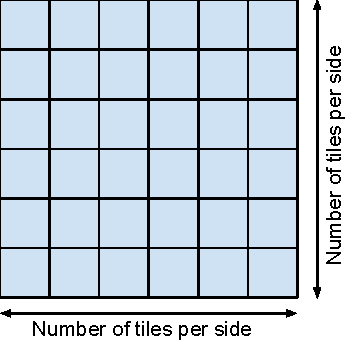
\includegraphics[width=\linewidth]{figures/design_space/spatial/static_partitioning.pdf}
  \caption{Illustration of partitioning geographical space using the static partitioning technique.}
  \label{fig:static_part}
\end{subfigure}%
~~~~~~~~
\begin{subfigure}{0.6\textwidth}
  \centering
  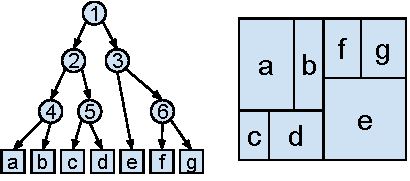
\includegraphics[width=\linewidth]{figures/design_space/spatial/kdtree_partitioning.pdf}
  \caption{Illustration of partitioning geographical space using the KD-Tree technique.}
  \label{fig:kdtree_part}
\end{subfigure}\par\medskip
\caption{Illustration of the candidate spatial partitioning approaches evaluated in the design space exploration. In both the figures, the rectangular area represents the application's geographical coverage and each rectangle inside it represents a tile to which entities are mapped.}
\end{figure}

\begin{itemize}
\item \textbf{Static Partitioning}. Similar to GeoHash, this geo-indexing technique statically divides the  geographical space into a number of tiles. Since we are not interested in the numeric value of the tile's identifier (unlike typical use-cases of geo-indexing approaches such as GeoHash), we simplify the partitioning by assuming that geographical space is partitioned into a grid of squares, and the side length of each square is configurable. Each tile can then be represented by a tuple $\left( row, col \right)$, where $row$ and $col$ represent the position of the tile in the grid. Given the location of a client, it is straightforward to map it to a tile based on the size of each tile and the size of the total geographical area.
\item \textbf{KD-Tree based Partitioning} uses a two-dimensional KD-tree to partition geographical space. The vertices in the KD-tree represent geographical areas, with the root vertex representing the entire geographical space in question, while the leaf vertices represent the tiles. The spatial bounds of a vertex are fixed and decided when creating the vertex. Looking up the tile that a given client belongs to requires performing a traversal starting from the root vertex down to the leaf vertex that represents the actual tile. At each step in this traversal, the bounds of the child nodes and the given client's location are used to decide which of the child nodes to move to next. The size of each tile is not fixed, rather it changes dynamically as the tree is updated. The only constraint that is enforced by the tree is that the number of clients mapped to a specific tile should not exceed an \textit{occupancy threshold}. If the occupancy of a particular tile becomes higher than the threshold, the tile is split and two children tiles are created. Furthermore, if the total occupancy of two tiles that have the same parent tile is less than the occupancy threshold, the two child tiles are merged.
\end{itemize}

\begin{figure}
\centering
\begin{subfigure}{0.45\textwidth}
  \centering
  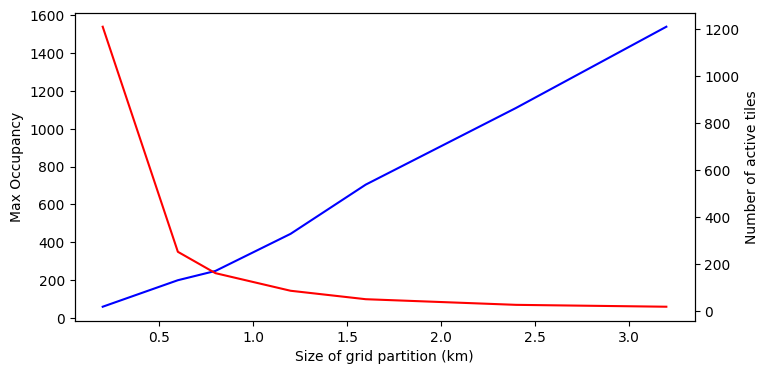
\includegraphics[width=\linewidth]{figures/design_space/spatial/metrics_Grid.png}
  \caption{Variation of metrics of interest for the static partitioning technique with varying size of each partition.}
  \label{fig:static_part}
\end{subfigure}
~~~~
\begin{subfigure}{0.45\textwidth}
  \centering
  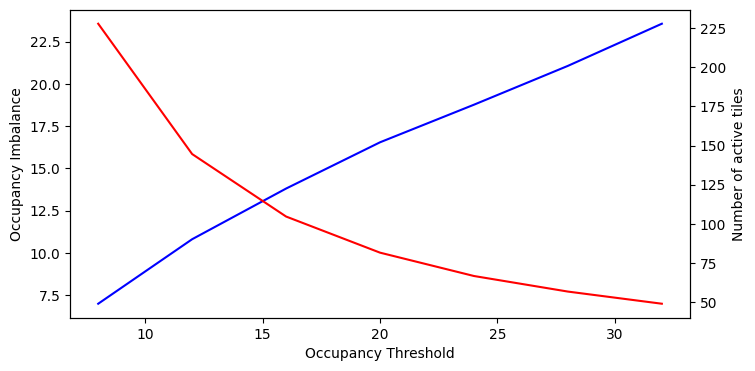
\includegraphics[width=\linewidth]{figures/design_space/spatial/metrics_KDTree.png}
  \caption{Variation of metrics of interest for the KD-Tree based dynamic spatial partitioning technique with changing occupancy threshold per tile.}
  \label{fig:kdtree_part}
\end{subfigure}\par\medskip
\end{figure}

We first evaluate the performance of the Static Partitioning technique against the aforementioned client workload. We evaluate the two metrics of interest - namely Maximum Occupancy and Number of Active Tiles. The evaluation is done with several different configurations of each partitioning technique. \cref{fig:static_part} shows the variation of the maximum occupancy and the number of active tiles as a function of the side-length of each geographical partition. As the size of the grid partition increases, the maximum occupancy grows, along with a decrease in the number of active tiles. This tradeoff is shown in \cref{fig:spatial_tradeoff} as well.
\par Next we perform the same experiment with the KD-Tree based spatial partitioning technique, wherein we configure the Occupancy Threshold for each tile. We vary the occupancy threshold from 8 to 32 and plot the metrics of interest in \cref{fig:kdtree_part}. The metrics show a similar behavior as in \cref{fig:static_part}. As the occupancy threshold increases, the number of active tiles that exist in the system decreases, because each tile can hold more clients. In addition, the increase of occupancy threshold also results in higher maximum occupancy in the system.

\begin{figure}
\centering
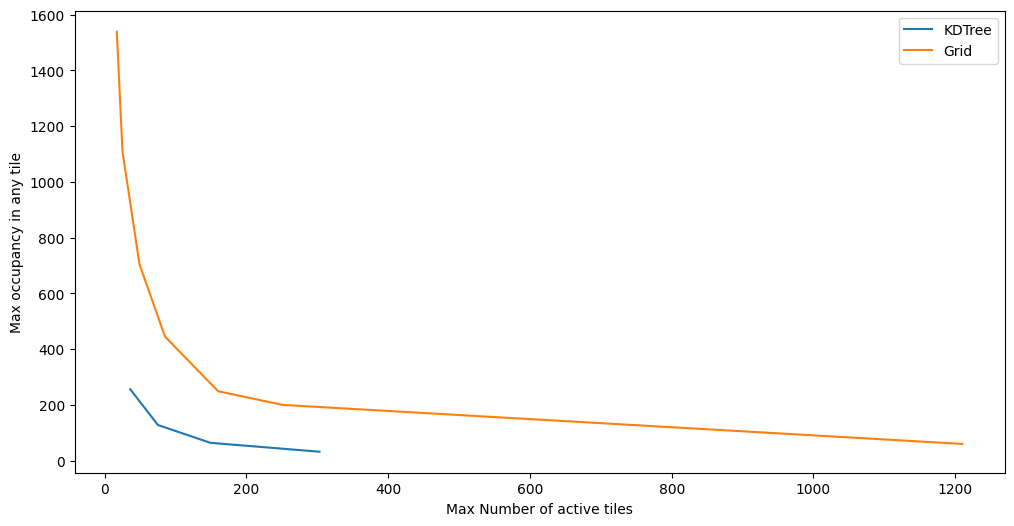
\includegraphics[width=0.75\linewidth]{figures/design_space/spatial/spatial_partitioning_tradeoff.png}
\caption{Tradeoff between the two metrics of interest - Maximum Occupancy and Number of Active Tiles - for the two types of partitioning techniques evaluated. We changed the configuration of each partitioning technique and repeated the experiment to obtain a range of performance output, that shows the tradeoff between the two metrics.}
\label{fig:spatial_tradeoff}
\end{figure}

\cref{fig:spatial_tradeoff} shows the tradeoff between the two metrics of interest for the two spatial partitioning techniques that we evaluate. Both the partitioning techniques show similar behavior in the tradeoff curve, where an increase in maximum occupancy results in a decrease in the number of active tiles, and vice versa. However, the absolute values of both the metrics are much lower for the KD-Tree based partitioning than the Static partitioning. The KD-Tree partitioning outperforms Static partitioning because it builds tiles based on the physical distribution of clients, instead of being predefined as in the case of Static partitioning. Because of the adaptive nature of the KD-Tree partitioning, a smaller number of tiles are able to uniformly divide the clients. 
\par The dynamically splitting and merging spatial partitions in the KD-Tree based spatial partitioning does not take place in the critical path of control plane operations. It is triggered asynchronously by the control plane policy when an opportunity to split or merge a tile is identified. When splitting and merging, the cache on the client side is invalidated and they connect to a new application instance that is created at the time of triggering the split or merge. The clients that connect to the new application instance would experience some downtime, because the new instance would take some time to initialize. However, such an event does not occur frequently because split/merge operations are called in the event of spatial skews, which are infrequent. \cref{fig:spatial_ctx_client_downtimes} shows the distribution of client downtimes experienced in one of the scenarios from the experiment performed to evaluate the KD-Tree candidate design, where the occupancy threshold was set to 32. 
\begin{figure}
\centering
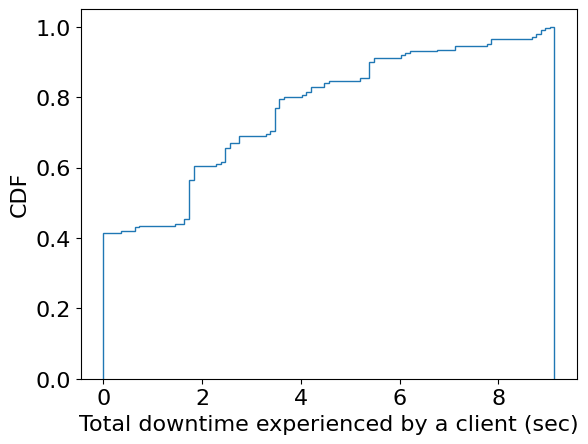
\includegraphics[width=0.5\linewidth]{figures/design_space/spatial/client_downtimes.png}
\caption{CDF of total downtime experienced by clients due to dynamic splitting and merging of spatial partitions by the KD-Tree based approach.}
\label{fig:spatial_ctx_client_downtimes}
\end{figure}
Hence, we choose KD-Tree based dynamic spatial partitioning technique for building the dynamic spatial context mechanism.
\subsection{Monitoring Client Location}
Monitoring the current location of clients is necessary for maintaining the KD-Tree based spatial partitioning because of two main reasons: (1) it provides the information necessary for maintaining the occupancy of entities in different tiles, and trigger the remapping of an entity to another tile when it leaves the current one; and (2) when partitioning a tile, updated entity locations provide hints about how to partition the tile so that a roughly equal number of entities are present in both the children tiles.
The metadata associated with the spatial partitioning is maintained in a centralized location that serves as the authoritative copy. Sending location updates from all clients to the centralized location consumes network bandwidth as well as creates a large number of occupancy updates that do not necessarily result in a change in the current tile. Hence, we conduct a design space exploration of the location monitoring module of this mechanism to find a design that lowers these overheads.
\subsubsection{Metrics of Interest}
We choose two metrics of interest for evaluating the candidate designs for the location monitoring module of the dynamic spatial context management mechanism. 
\begin{itemize}
\item \textbf{Messaging Overhead. } We measure the number of location monitoring messages that need to be sent to the centralized location that maintains the authoritative copy of the spatial partitioning metadata. This metric should be minimized to improve system scalability. 
\item \textbf{Total Occupancy Violation Time. } We measure the sum of all the time durations for which some tile's occupancy threshold is violated. Since the occupancy threshold is set by the application, violating it would result in a workload surge leading to performance degradation.
\end{itemize}

\subsubsection{Candidate Approaches Evaluated}
\begin{itemize}
\item \textbf{Centralized Approach. }A straightforward design for maintaining updated client locations is to send all location updates from clients to the centralized location holding the authoritative copy of the spatial partitioning. Clients receive the identifier of the current tile based on their current location, and if the received tile identifier is different from the current tile, they would connect to the application instance corresponding to the new tile. The centralized spatial partitioning unit would transparently handle scenarios when the partitioning is updated due to tile merging or splitting operations. Although this approach is very straightforward to design and implement, it suffers from high overhead of constantly monitoring the locations of all clients at all times.
\item \textbf{Distributed Approach. } Unlike the centralized approach, where the client simply reports the current location to the spatial partitioning module and receives the identifier of the current tile, the distributed approach maintains a cache of the spatial partitioning locally in the client library. The local cache is invalidated and updated every time the currently cached tile in the centralized authoritative copy is updated due to tile merging or splitting operations. The cache is then used by the client to keep track of its location with respect to the current tile, and when its location leaves the current tile, it triggers a migration to connect to the new tile. The cache also periodically reports its location to the authoritative copy so that tile split operations can effectively partition clients into the child tiles equally. The periodicity of reporting location to the control-plane is configurable, and it affects how uniformly clients are split among child tiles. We expect that with infrequent location updates from clients, the number of clients in child tiles as a result of a split operations would not be uniform, thereby increasing the likelihood of another occupancy threshold violation in the future.
\end{itemize}

\begin{figure}
\centering
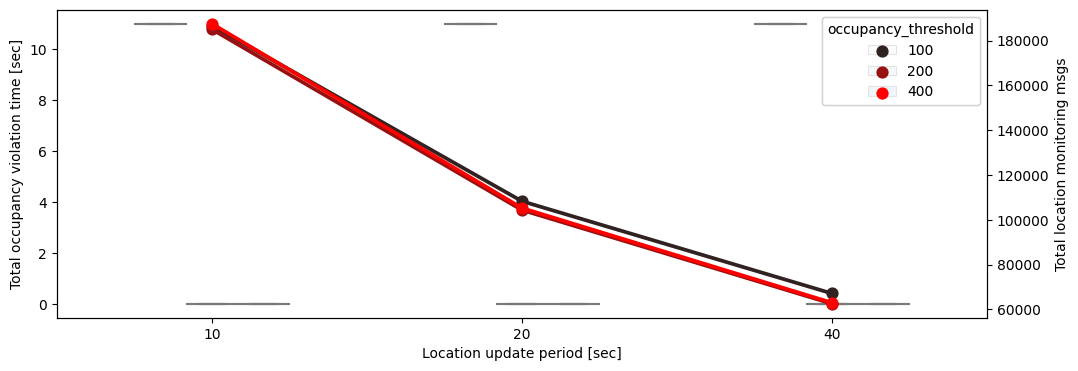
\includegraphics[width=\linewidth]{figures/design_space/spatial/loc_update_period_tradeoff.png}
\caption{Effect of location update period on the duration of occupancy violation faced by tiles and the amount of location monitoring messages that need to be sent to the control plane.}
\label{fig:location_update_period}
\end{figure}
\cref{fig:location_update_period} shows the variation of duration of occupancy violation and total number of location monitoring messages sent with increasing location update period. The increase in location update period does not have any noticeable impact on the violation duration, however it results in a significant drop in the number of messages for monitoring location of clients. Since the client immediately sends a location update when it leaves the current tile irrespective of the location update period, the violation duration is not dependent on location update period. In fact, for an occupancy threshold of 200, the violation duration is 0, that shows that there are no occupancy violations. Hence, choosing a high location update period does not significantly impact the total violation duration, but significantly reduces location monitoring traffic.

\section{Network Proximity Estimation}
\label{sec:nw_prox_dse}
Control-plane policies of platform services need to make data and compute placement decisions so as to satisfy data processing latency constraints. In an Edge setting, network communication latency forms a significant portion of the end-to-end latency. Previous works in the cloud computing domain have come up with accurate techniques for estimating computation latency, but did not consider communication latency due to the rather homogeneous and well connected nature of datacenter network topologies. In an Edge infrastructure, it is important to be able to accurately estimate the network latency between a pair of system entities, so that the control plane policy can take a data/compute placement decision to satisfy end-to-end latency.
\par Network proximity estimation cannot be done using active measurements at the time of execution of the control plane policy logic, because a typical policy evaluates several candidate nodes (such as selecting the best candidate for application placement) and therefore  requires pairwise network latency between several pairs of nodes to take its decision. Waiting for the measurements to complete in the critical path of policy execution would severely impact the responsiveness of the control plane. Hence, the network proximity estimation mechanism needs to continuously maintain network proximity metadata for each node in the infrastructure. The size of the metadata needs to be tractable so that it can be efficiently queried to estimate pairwise network latency.
\par The mechanism should estimate pair-wise network latency with high accuracy. Furthermore, it should be able to quickly adapt to changes in network topology due to client mobility or link failures. Both the accuracy and recovery-time of the mechanism to topology dynamism should not deteriorate with increasing number of nodes, meaning that the mechanism should be scalable.

\subsection{Metrics of Interest}
We consider the following metrics of interest when evaluating the candidate design choices for network proximity estimation mechanism.

\begin{itemize}
\item \textbf{Latency Estimation Error.} We measure the root-mean squared error between the estimated and the actual (ground-truth) network latency. For a pair of nodes $i$ and $j$, the estimated and actual network latencies for the pair $\left( i, j\right)$ is denoted by $N_{\left( i, j\right)}$ and $\hat{N}_{\left( i, j\right)}$, respectively. The root-mean squared error (RMSE) in latency estimation is then calculated as shown in \cref{eq:rmsre}.
\begin{equation}
\label{eq:rmsre}
RMSE = \sqrt{\sum_{\forall \left(i, j \right) i \neq j}{\left(N_{\left( i, j\right)} - \hat{N}_{\left( i, j\right)}\right)^2}}
\end{equation}
\item \textbf{Number of Messages Exchanged}. We measure the number of messages exchanged between the various nodes in the system before the error in latency estimation drops below the maximum threshold.
\item \textbf{Amount of Metadata} needed by control-plane policies. We analytically calculate the amount of information that would need to be stored at the control plane in order to support a typical compute/data placement policy.
%\item \textbf{Response-Time to Topology Dynamism.} We measure the amount of time taken after a change in a particular node's connectivity before all the nodes are aware of that change. This measures the response-time of the mechanism to react to topology changes.
\end{itemize}

\subsection{Candidate Design Choices Evaluated}
\begin{figure}
\centering
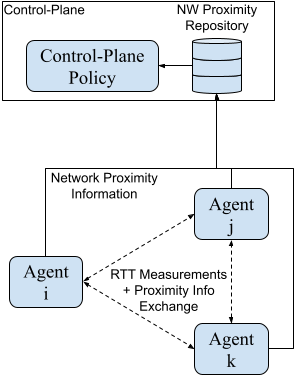
\includegraphics[width=0.4\linewidth]{figures/design_space/nw_prox/basic_sys_arch.png}
\caption{Basic components in the system architecture of the network proximity estimation mechanism. Multiple participating agents communicate among each other to perform actual RTT measurements and compute network proximity, and share the proximity information with one another. The network proximity information is uploaded to a repository in the control plane from where this information is supplied to control plane policies.}
\label{fig:nw_prox_arch}
\end{figure}
\cref{fig:nw_prox_arch} shows the basic architecture that the various design choices of the network proximity estimation mechanism have. It is composed of a number of \textit{agents}, with one agent co-located with every system entity with which network proximity needs to be measured. Each agent computes its network proximity to the other agents, and communicates the proximity information to a central repository, that is queried by control-plane policies for estimating network round-trip time (RTT) between any two system entities. The design choices that we explore in this section follow the agent-based architecture, and differ in the kind of communication protocol that each agent follows and the kind of metadata stored by the mechanism that allows it to answer network proximity queries. We evaluate the following design choices for the network proximity estimation mechanism. 
\subsubsection{Pair-wise Measurements based Approach}
In this approach, representation of network proximity is in the form of a 2-dimensional array $A$, where $A [ i, j ]$ represents the network latency between agent $i$ and $j$. Each participating agent periodically performs a network round-trip time (RTT) measurement between itself and another agent. Each agent uses a round-robin policy to select which other agent it is going to probe to measure the RTT. After each measurement, the agent provides the RTT information between itself and the other agent with which the measurement was performed to the centralized repository of network proximity.

\subsubsection{Network Coordinates}
Network coordinate (NC) systems are distributed protocols to scalably determine the network proximity between a pair of nodes in a distributed system without performing direct measurements \cite{donnet2010survey} between all pairs of nodes. Such systems embed nodes in a geometric space such that the network latency between any two nodes can be estimated by calculating the Euclidean distance between their positions (coordinates) in this space. Previous work on analysis of latencies in the Internet has shown that nodes can be embedded in a 3-dimensional or higher space with relatively high accuracy of network proximity estimation \cite{lee2009suitability}.
\par \noindent \textbf{Embedding in $d$-dimensional space. } Each agent $i$ maintains a network coordinate $x_i$ that is an $d$-dimensional vector. Each agent $i$ periodically performs an RTT measurement with another agent $j$ and also fetches the current network coordinate of agent $j$, that we denote as $x_j$. By using the measured actual RTT $rtt_{i,j}$ between itself and the other agent $j$, the given agent $i$ updates its own network coordinate so as to reduce the error of latency estimation. To do so, agent $i$ first calculates the error in latency estimation, as shown in \cref{eq:rtt_err}.
\begin{equation}
e = rtt_{i,j} - || x_i - x_j ||
\label{eq:rtt_err}
\end{equation}
Each iteration of this coordinate update process at agent $i$ aims at applying a force on $x_i$ so as to move it toward its correct position in the $d$-dimensional space with respect to agent $j$'s coordinate. In other words, if the error calculated in \cref{eq:rtt_err} is positive, $x_i$ would be pushed away from $x_j$, otherwise it will be pulled closer to $x_j$. This notion is captured in \cref{eq:nc_force}, that computes the unit vector of the force to be applied to $x_i$.
\begin{equation}
dir = u \left( x_i - x_j \right) 
\label{eq:nc_force}
\end{equation}
The force that needs to be applied to coordinate $x_i$ is in the direction of the unit vector in \cref{eq:nc_force} and has the magnitude proportional to the error in \cref{eq:rtt_err}. $x_i$ is then updated in the direction of the force by a small and configurable amount.
\begin{equation}
x_i = x_i + \delta \cdot e \cdot dir 
\label{eq:nc_update}
\end{equation}

\par \noindent \textbf{Capturing Access Link Delays. } A number of hosts connected to the Internet today do so behind access links. While the $d$-dimensional Euclidean space is good at modeling latencies in the Internet core, incorporating a scalar $height$ component in the network coordinate significantly improves the network RTT estimation error \cite{vivaldi}. The height component represents the network latency incurred to traverse the access link beyond which latencies can be estimated using the Euclidean coordinate system. The estimated RTT between two agents $i$ and $j$ with combined network coordinates $\left( x_i, height_i \right)$ and $\left( x_j, height_j \right)$ respectively is given by $|| x_i - x_j || + height_i + height_j$. This equation captures the fact that for packets to travel from agent $i$ to $j$, they first have to traverse the access link of agent $i$, travel through the Internet core toward agent $j$ (that can be modeled using Euclidean distance), and then traverse the access link of agent $j$. 

\par \noindent \textbf{Reducing Errors due to Triangle Inequality Violations. } Internet topologies frequently violate the triangle inequality that should ideally hold in a Euclidean space. The triangle inequality requires that the sum of the RTT between agents $i$ and $j$ and that between agents $j$ and $k$ should be greater than the RTT between agents $i$ and $k$. This inequality is violated in real-world network topologies because of heterogeneous routing policies \cite{zheng2005internet}. However, Lee et al. \cite{lee2009suitability} found that such violations occur more frequently  among nodes that are at closer network distances from one another. Hence, they introduce a scalar $adjustment$ term in the network coordinate to account for the non-Euclidean effect due to triangle-inequality violations. The adjustment term is calculated as shown in \cref{eq:adjustment}, where $n$ represents the number of measurements taken.
\begin{equation}
adj_i = \dfrac{1}{2} \cdot \dfrac{\sum_{j} rtt_{i,j} - || x_i - x_j ||}{n}
\label{eq:adjustment}
\end{equation}

\par We employ a popular decentralized network coordinate protocol, Vivaldi \cite{vivaldi} with some enhancements proposed by Ledlie, et al.~\cite{ledlie2007network} and Lee, et al.~\cite{lee2009suitability}. Prior art has shown that network coordinate protocols provide efficient, accurate, and stable latency estimates in the wild~\cite{ledlie2007network}.

\subsection{Evaluations of Candidate Design Choices} 
We evaluate the performance of the candidate design choices for implementing the network proximity estimation mechanism and present the results in this section.

\subsubsection{Accuracy of Network RTT Estimation}
\label{sec:nw_rtt_error}
The network proximity estimation mechanism is expected to accurately estimate network RTT between agents in a real-world geo-distributed infrastructure topology. We use the topology of Edge sites belonging to Alibaba Edge Node Service \cite{xu2021cloud}, that has sites deployed all across mainland China. The dataset provides city-level location of Edge sites along with the actual network RTT between them. In this experiment, in addition to evaluating the error of RTT estimation, we also intend to study how the scale of the infrastructure topology affects the error. We build infrastructure topologies of increasing scale by selecting the top-k cities with the most edge sites and only considering the sites in those cities. Each site runs an agent of the network proximity mechanism, and communicates with potentially every other Edge site to collect RTT and update its network proximity model.
\par \cref{fig:nw_coord_error} shows the evolution of the error in RTT estimation over time for network topologies of increasing scale. The root-mean squared error of latency estimation does increase with an increase in the scale of the network topology, but it converges at around 4.5ms in RTT estimation, which is a reasonable error rate given the variance in ground-truth latency measurements. We do not evaluate accuracy of the pairwise measurements based approach, because the RTT estimates are simply an aggregation of the previously measured RTT values, and hence it would always result in very low error. \begin{figure}
\centering
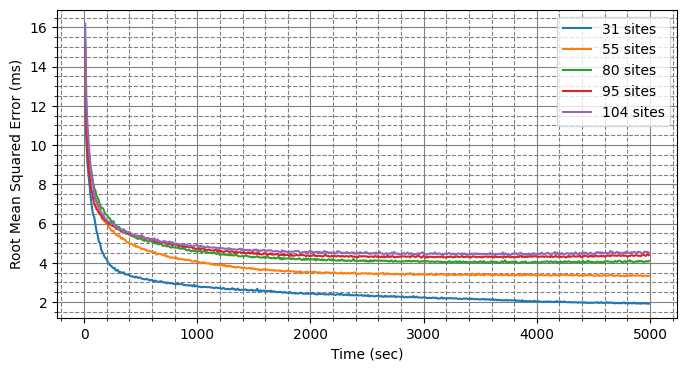
\includegraphics[width=0.75\linewidth]{figures/design_space/nw_prox/error.png}
\caption{Evolution of error in RTT estimation for the network coordinate-based design. The figure shows the RTT estimation error for network topologies of increasing scale.}
\label{fig:nw_coord_error}
\end{figure}

\subsubsection{Communication Overhead}
We now evaluate the amount of communication that needs to happen between the agents of the network proximity estimation mechanism in order to build a reasonably accurate inter-agent network RTT estimation model. We compare the number of messages that need to be communicated between the agents for both the pairwise measurement and network coordinates based designs of the mechanism. 
\par For this experiment, we intend to evaluate network topologies of much larger scale than the Alibaba Edge Node Service topology used in \cref{sec:nw_rtt_error}. We adopt a hub-and-spoke model for generating a synthetic topology for this experiment, with each spoke having a network latency uniformly sampled between 10 and 60 ms. We choose such a model for building the topology because it offers a simple way to model random network characteristics between different pairs of nodes. Each node in the topology runs an agent of the network proximity estimation mechanism. The number of nodes in the topology is varied to evaluate the design choices at different scales.
\begin{figure}
\centering
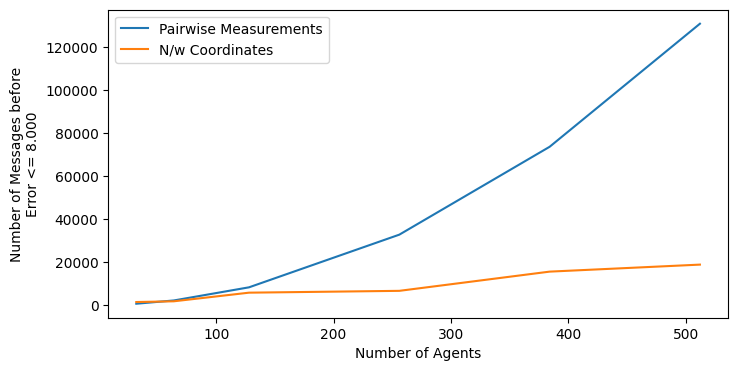
\includegraphics[width=0.75\linewidth]{figures/design_space/nw_prox/comm_overhead.png}
\caption{Communication overhead of the two design choices for network proximity estimation mechanism. The pairwise measurement based design requires $O \left( n^2 \right)$ communication rounds, whereas the communication rounds needed by the network coordinates based approach scales almost linearly.}
\label{fig:comm_overhead}
\end{figure}

\par \cref{fig:comm_overhead} shows the number of communication rounds that need to take place (combined over all nodes) before the network proximity estimation mechanism's error falls below a threshold of 8 milliseconds. The pairwise measurement approach needs to measure the network latency between all pairs of nodes, meaning that it requires $N \left( N - 1 \right)$ rounds of communications, that grows quadratically with increasing number of nodes. On the other hand, the network coordinates approach grows almost linearly, because it only tries to embed nodes in a high-dimensional space based on a small set of measurements. Hence, the network coordinates based approach is a more scalable design for network proximity estimation.

\subsubsection{Size of Network Proximity Repository}
Control-plane policies would frequently query the centralized repository of network proximity estimation to obtain the RTT between a pair of agents. A large metadata would mean that the query would take longer to execute, hence, reducing the speed of control-plane policy execution. We compare the amount of metadata to be stored for the two design choices. 

\begin{figure}
\centering
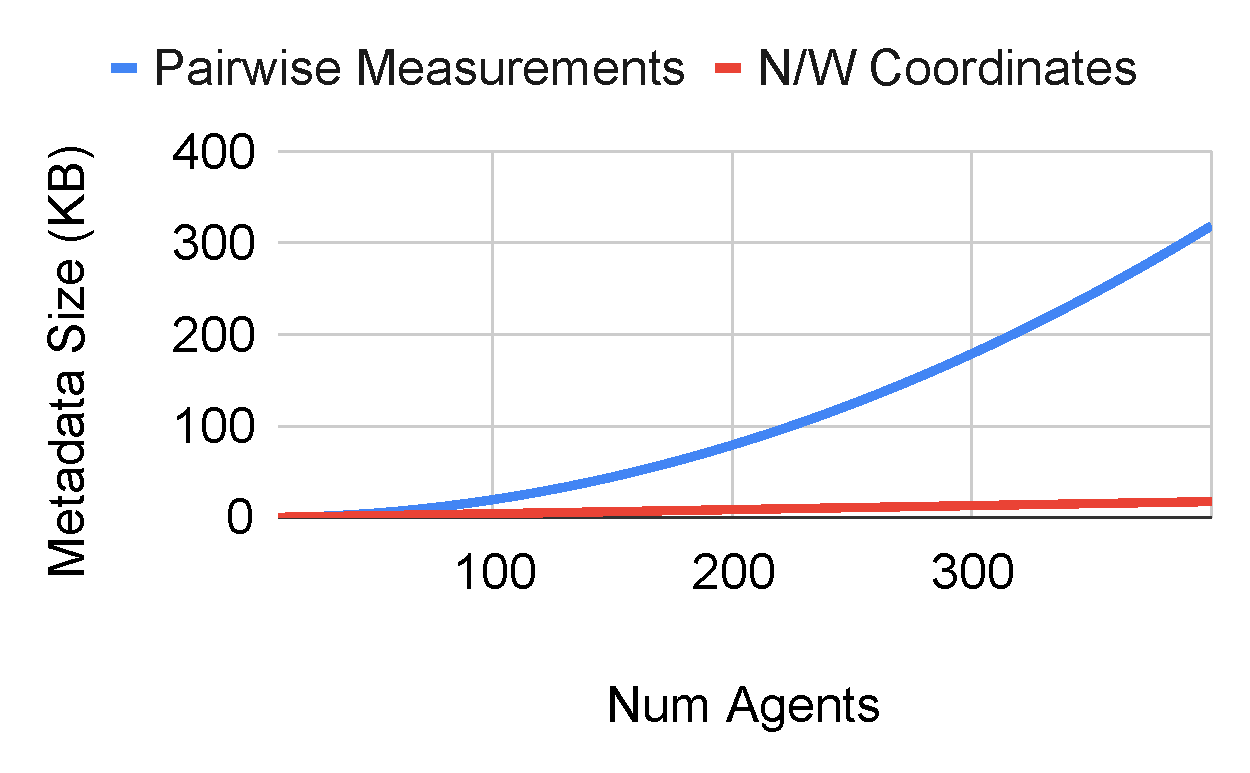
\includegraphics[width=0.75\linewidth]{figures/design_space/nw_prox/metadata_size.pdf}
\caption{Comparison of the size of network-proximity metadata that needs to be stored at the control-plane.}
\label{fig:metadata_size}
\end{figure}

\par \cref{fig:metadata_size} shows how the metadata size grows with increasing number of agents. Since the pairwise measurements based design would need to store the network latency between each pair of agents, the size of the metadata grows quadratically. However, the metadata for the network coordinates based approach consists of one coordinate per agent, that amounts to 44 bytes and grows linearly.

\subsection{Running Network Coordinate Agents on Mobile Clients}
Client mobility results in the change of network routing between client and the Edge infrastructure, since the network access point to which the client is connected changes. The change of network access points results in a change in network latencies to reach the Edge sites, that affects the ground-truth on which the network coordinates protocol relies for converging to stable coordinates. The end result of these perturbations is a deterioration of the RMSE of network latency estimation, that is shown in \cref{fig:mobility_nc_rmse}. To evaluate the performance of the network coordinates protocol used in the Network Proximity Estimation mechanism, we evaluate the protocol with varying degrees of client mobility. Client mobility affects network coordinates protocol primarily by continuously changing the network access point used by clients to connect to the Edge infrastructure. Hence, we emulate different speeds of client mobility by controlling the average time between network access point changes for each client. The time between two consecutive access point changes for a client is sampled from an exponential distribution with the mean of the distribution set as mentioned above.
\begin{figure}
\centering
\begin{subfigure}{0.48\textwidth}
  \centering
  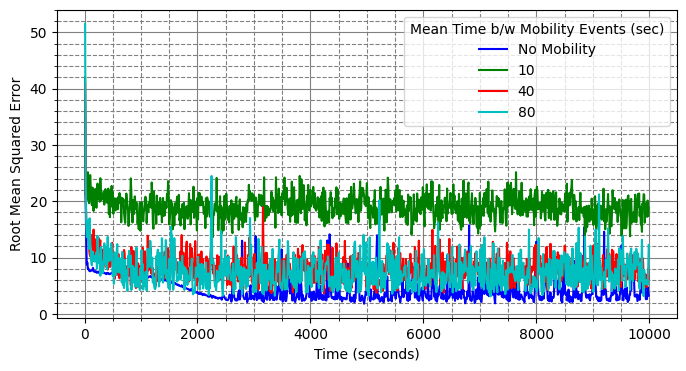
\includegraphics[width=\linewidth]{figures/design_space/nw_prox/rmsre_vs_time_num_agents_64.png}
  \caption{64 Clients.}
  \label{fig:mobility_N_64}
\end{subfigure}
\begin{subfigure}{0.48\textwidth}
  \centering
  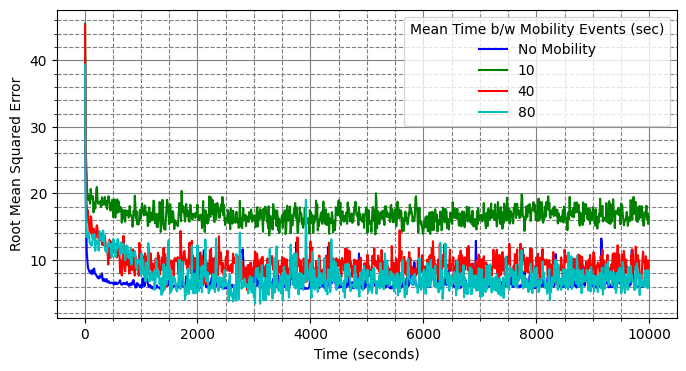
\includegraphics[width=\linewidth]{figures/design_space/nw_prox/rmsre_vs_time_num_agents_256.png}
  \caption{256 Clients.}
  \label{fig:mobility_N_256}
\end{subfigure}
\begin{subfigure}{0.48\textwidth}
  \centering
  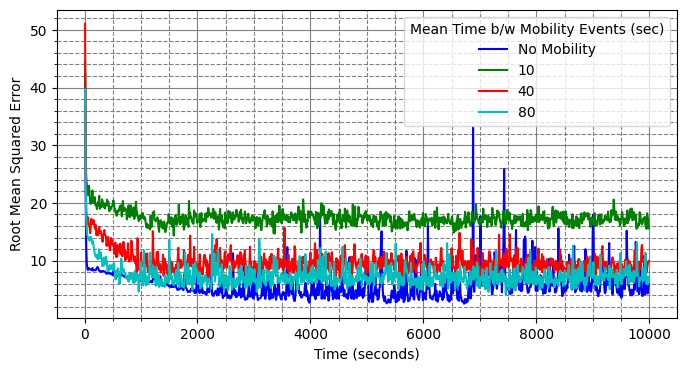
\includegraphics[width=\linewidth]{figures/design_space/nw_prox/rmsre_vs_time_num_agents_512.png}
  \caption{512 Clients.}
  \label{fig:mobility_N_512}
\end{subfigure}
\caption{Variation of RMSE over time for varying number of clients and varying degrees of client mobility.}
\label{fig:mobility_nc_rmse}
\end{figure}
For all scenarios with different number of clients, the RMSE in network latency estimation is the lowest for the case without mobility and increases progressively with more frequent mobility events per client. Hence, we conclude that the frequent changes in network connectivity for clients results in deterioration of RMSE of network latency estimation. Therefore, we propose an approach to eliminate this error in the following subsection.

\subsubsection{Network Coordinate Proxy running on Edge Gateway}
Mobile devices invariably connect to the Internet via a nearby gateway node that runs on the Edge of the network e.g., local breakout \cite{localbreakout} for clients running on a 4G/LTE network. We assume the presence of a lightweight network coordinate proxy (NC Proxy) running on such a gateway node, serving as the source of network coordinate information for the mobile clients connected to that gateway node. For a client that is connected to the Internet via a particular Edge gateway, all uplink and downlink traffic flows through that gateway, and it is located at a fixed access network latency from the client. Hence, the network latency between the client and an Edge site can be calculated by computing the sum of the network latency between the site and the Edge gateway and the access latency between the client and the gateway. Therefore, the network coordinate agent on the mobile client computes its current coordinate by using the vector and adjustment fields of the gateway's coordinate, and adding the access latency to the height component of the gateway's coordinate. The access latency is monitored by periodic measurement from the gateway. It is noteworthy that the number of such network coordinate proxies is going to be much smaller than the number of clients -- because each proxy serves a large number of clients. Hence aforementioned strategy for calculating network proximity is not only more stable for mobile clients, but also more scalable. 

\par In this dissertation, we assume that the accurate discovery of the network coordinate agent running on the current serving Edge gateway can be facilitated by a DNS-based mechanism. Such a mechanism for application-level resolution at the Edge has been already presented in the context of content-delivery networks \cite{hsu2020dns}. 

\section{Distributed End-to-End Monitoring}
\label{sec:e2e_mon_dse}
The data-plane of applications using a platform service usually comprises multiple components, with each component performing a specific action, and incurring latency. The latency incurred by each such component adds toward the end-to-end latency of the application, that is expected to be lower than a certain threshold by the developer. Hence, the end-to-end monitoring mechanism aims to provide the ability to monitor the end-to-end latency of the data-plane for a variety of applications running on different platform services. We propose to do so by measuring all individual component latencies independently. The collected metrics are then aligned with respect to time using their timestamps and summed up to compute the end-to-end latency. The end-to-end latency estimate can then be used to check whether the constraints specified by developer have been violated. In the case of detecting a violation, the individual component latencies are used for performing a root-cause analysis to detect the component latency that is the source of the violation.

\subsection{Logical Components in the Monitoring Mechanism}
\label{sec:monitoring_functions}
\begin{figure}
\centering
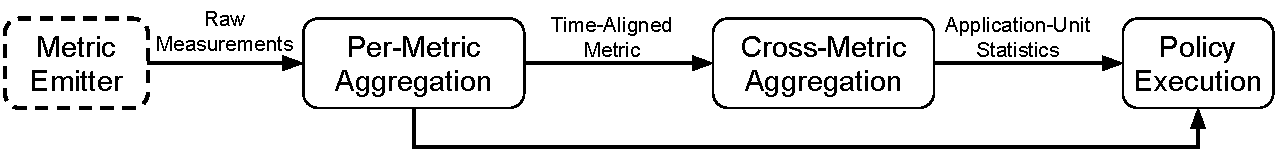
\includegraphics[width=\linewidth]{figures/design_space/monitoring/functions.pdf}
\caption{Logical components in the end-to-end monitoring mechanism and their interactions.}
\label{fig:monitoring_functions}
\end{figure}
\cref{fig:monitoring_functions} shows the logical functions that we propose as a part of the end-to-end monitoring mechanism. These functions perform all the necessary actions that are needed by typical platform services in order to continuously serve applications' desired quality of service.
\subsubsection{Metrics Emitter}
The Metrics Emitter component represents the platform service component generating measurements for a metric. The Metric Emitter could be the client library on a certain client device, an application instance or a platform service component running on an Edge site. 
\subsubsection{Per-Metric Aggregation}
The Metrics Emitter generates raw measurements that are processed by the Per-Metric Aggregation function, that time-aligns the metric measurements while performing an aggregation as well to reduce the data volume. The output of the per-metric aggregation component is a stream of time-aligned measurement values that are emitted at regular intervals. The time interval between two consecutive measurements emitted by the per-metric aggregation component is equal to the bucket-size parameter of the time-alignment process. The timestamp associated with each aggregated time-aligned measurement values in the output stream is the start timestamp of the bucket.

\subsubsection{Multi-Metric Aggregation}
The Multi-Metric Aggregation function takes multiple time-aligned metrics at a particular timestamp as input and runs a platform-specific function to generate an aggregated value for that timestamp. 

\subsubsection{Policy Execution}
The control-plane policies then read the aggregated statistics generated by multi-metric aggregation as well as the time-aligned metrics to make decisions such as whether a certain application instance is undergoing performance violation and subsequently determining the root-cause of the violation.

\subsection{Design of the core components of end-to-end monitoring mechanism}
\subsubsection{Metrics Agent}
The Metrics Agent component is the one that is deployed alongside application and platform service components that need to be monitored, and acts as the interface between the system components and the monitoring system. It is deployed as part of the client library or the application runtime or as a side-car of the platform service components. It provides interfaces for application and platform service components to register metrics and record observations for those metrics. 

\subsubsection{Metrics Server}
The Metrics Server is the component that holds the metrics reported by the various Metrics Agents. The Metrics Server serves two main functions - (i) it acts as a store for time-series measurement values, and (ii) an execution runtime for the aggregation and policy functions as discussed in \cref{sec:monitoring_functions}. 
\par The Metrics Server provides an interface similar to a Time-Series Data Base (TSDB). The Metrics Server provides a relational schema for defining metrics and their associated metadata. Having a relational schema also allows aggregation and policy logic to express queries based on metadata fields. The Metrics Server supports high-velocity ingestion of observations, and efficient support for querying historical metric values.
\par The Metrics Server supports platform-specific functions to be executed over the monitoring data that is stored in its data store. It allows the aggregation and policy functions to query metrics using their metadata fields. Once the identifier for a particular metric is known, the Metrics Server allows queries to fetch most recent as well as historical measurements recorded for that metric.

\subsection{Metrics of Interest}
We consider the following metrics of interest for quantifying the \textit{goodness} of the various design choices for implementing the end-to-end monitoring mechanism.
\begin{itemize}
\item \textbf{Monitoring Traffic through WAN. } The large number of application and platform-service entities continuously processing data and generating performance metrics would present a large volume of data to be fed into the monitoring system. The amount of traffic sent through the WAN needs to be minimized for the mechanism to be scalable.
\item \textbf{Detection Latency of Violation. }The time taken by the monitoring subsystem (including the Policy) to detect a significant change in a metric defines the responsiveness of the platform service to alleviate a potential violation. Hence, we intend to minimize the time taken by the monitoring mechanism to detect a violation.
\item \textbf{Resource Requirements of Metrics Server. } The CPU and memory usage of the monitoring components need to be low so that instances of Metrics Agents and Metrics Servers can be hosted on Edge resources. A high resource requirement would mean that resources that could have been used for the data-plane of platform services would need to be devoted to monitoring, potentially resulting in worse utilization of scarce Edge resources.
\end{itemize}


\subsection{Design Choices}
We explore two design choices for organizing the logical functions discussed in \cref{sec:monitoring_functions} over a geo-distributed infrastructure. We consider two design choices.

\subsubsection{Fully Centralized Approach}
In the fully centralized approach, all of the monitoring functionalities, ranging from the Per-Metric Aggregation to the Policy Execution are hosted in the Cloud. In this approach, the metrics are emitted by Metric Emitters located at the Edge within Metrics Agents, and the raw measurements traverse through the WAN to get to the downstream functions. 

\subsubsection{Distributed Approach}
In this approach, the Metric Emitters are located within Metrics Agents, that is same as the centralized approach. In addition to that, the Per-Metric Aggregation function for a given metric is co-located with the Emitter for that metric. In this way, raw measurements are not sent through the WAN, rather it is the time-aligned metric stream that is sent to the Cross-Metric Aggregation function. Since the bucket-size configuration parameter of a Per-Metric Aggregation instance does not change frequently, it is possible to maintain several geo-distributed instances at a large scale without the overhead of reconfiguring them frequently.

\begin{comment}
\subsubsection{Distributed Approach 2}
This approach is a variant of the Distributed Approach 1, wherein, the Cross-Metric Aggregation component is also moved to the Edge. Typical control-plane policies such as violation detection operate independently on a specific unit of the application, such as a specific application pipeline instance or publish-subscribe topic. Hence it is possible to host multiple instances of cross-metric aggregation component for different application units at multiple Metrics Servers running on the Edge. All the metrics corresponding to a specific application unit will need to be sent to the Metric Server that hosts that application unit's cross-metric aggregation function. 
\end{comment}

\subsection{Evaluation of Candidate Design Choices}
We evaluate the aforementioned candidate design choices for implementing the end-to-end monitoring mechanism and present results in this section. In our evaluations, we consider one application unit that has a number of distributed system entities associated with it. Each of these system entities generate measurements to one metric at a certain measurement frequency. Each metric is time-aligned using a specific bucket-size wherein the measurements falling inside a bucket are summarized by taking an average. The time-aligned summaries of each metric are sent to the Multi-Metric Aggregation that checks if all the metric summaries for the current bucket have been received, and if so, passes them to the policy execution component. 
\par In our experiments, the Metric Emitters are located on the Edge, while the Multi-Metric Aggregation is deployed in the Cloud. Per-Metric Aggregation can run either on the Edge alongside Metric Emitters or in the Cloud based on the design choice being evaluated. 

\begin{figure}
\centering
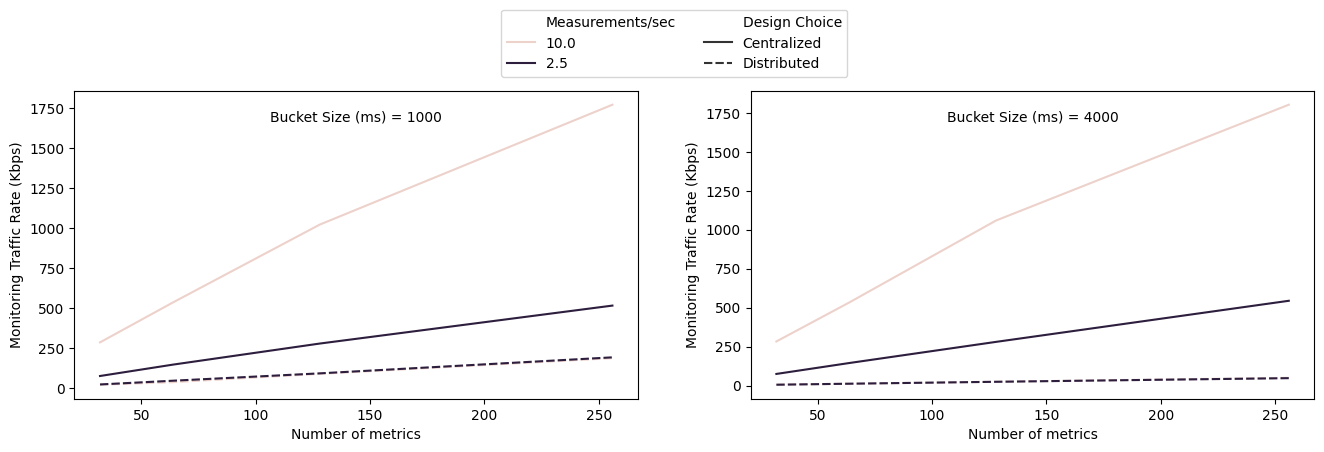
\includegraphics[width=\linewidth]{figures/design_space/monitoring/nw_usage.png}
\caption{Network bandwidth usage of the design choices for end-to-end monitoring mechanism.}
\label{fig:monitoring_nw_usage}
\end{figure}
\cref{fig:monitoring_nw_usage} shows the network bandwidth usage by the two design choices we evaluate for the end-to-end monitoring mechanism. We perform the evaluation for two bucket sizes - 1 second and 4 seconds - and two per-metric measurement rates - 2.5 and 10 measurements per second. For all four of these configurations, we see that the Distributed design choice incurs less network traffic between the Edge and the Cloud as compared to the Centralized design choice. Furthermore, the traffic consumed by Distributed approach does not change with different per-metric measurement rates because it only sends a summary of measurements (average) at an interval of 1 bucket size. This result quantitatively affirms our intuition that the Distributed design would be more scalable in terms of network bandwidth usage.

\begin{figure}
\centering
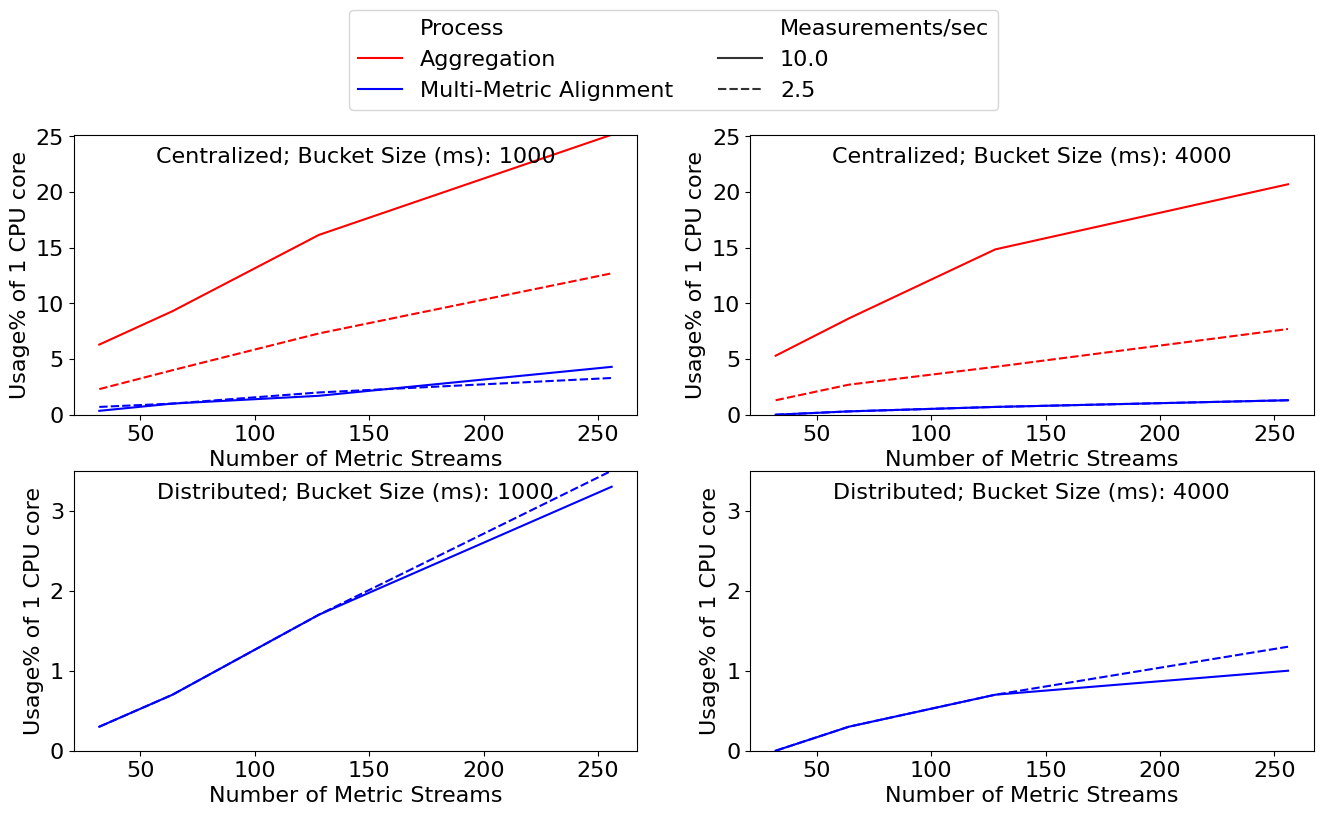
\includegraphics[width=\linewidth]{figures/design_space/monitoring/cpu_usage.png}
\caption{CPU usage of each component in various design choices of the end-to-end monitoring mechanism.}
\label{fig:monitoring_cpu_usage}
\end{figure}
\cref{fig:monitoring_cpu_usage} shows the CPU usage of the various components involved in the monitoring mechanism, when deployed in the evaluated design choice configurations. In the centralized approach, when all raw measurements are sent directly to the Cloud, the Per-Metric Aggregation components consume a high amount of CPU to process the incoming measurements. The CPU usage naturally grows with the number of metrics and the rate of measurements reported for each individual metric. The Multi-Metric Alignment component, however, is much less resource-intensive in comparison. In the Distributed approach, since the Per-Metric Aggregation component is co-resident with the Metrics Emitter, the CPU load for aggregating metrics is spread over all the geo-distributed Metric Emitters, and hence we do not show it in the figure. The evaluation results show that in terms of CPU usage, the Distributed design choice is more scalable.

\begin{figure}
\centering
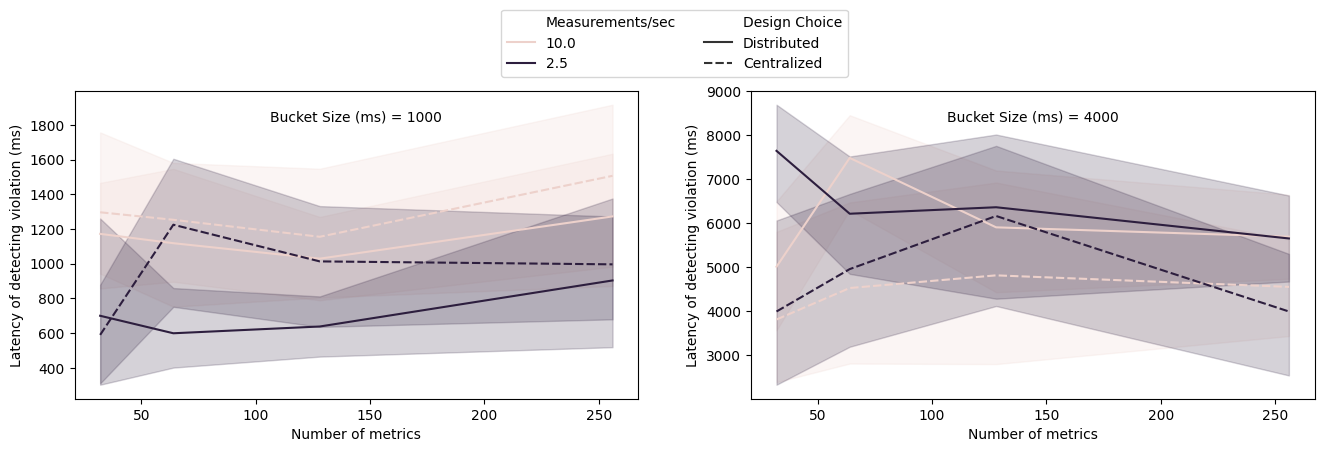
\includegraphics[width=\linewidth]{figures/design_space/monitoring/response_time.png}
\caption{Variation of the latency of detecting violations with the different design choices evaluated.}
\label{fig:monitoring_response_time}
\end{figure}
Finally, \cref{fig:monitoring_response_time} shows the variation of the latency of detecting a violation with the two evaluated design choices. The results show that both Centralized and Distributed Approaches have a similar behavior in terms of the violation detection latency, with the latency being dependent only on the bucket size. 
\par Hence, we conclude that the Distributed Design choice is not only more scalable in terms of network and CPU usage, but it also provides the same response time as the Centralized approach. Hence, we use it in implementing the end-to-end monitoring mechanism.

\subsection*{Summary}
So far in this dissertation, we have determined the three mechanisms which are its main contributions. We have identified the right abstractions that they should offer to the control plane policies and performed a design-space exploration to identify the best design for each mechanism for an Edge infrastructure. The next step is to demonstrate the utility of the proposed mechanisms in constructing platform services that will be used by application developers in constructing platform services to serve situation-awareness applications. We do so through three platform services, that are enumerated as follows:
\begin{itemize}
\item \oneedge{} is an application orchestrator, specifically designed for situation-awareness application to operate on Edge infrastructure. \cref{sec:oneedge} describes \oneedge{} and its use of the three mechanisms for placement of applications on the infrastructure, mapping clients to application instances and monitoring the performance of deployed application instances.
\item \epulsar{} is a topic-based publish-subscribe system that provides guarantees on end-to-end message delivery latency. It is presented in \cref{sec:epulsar}. It leverages the network proximity estimation mechanism to place topics on brokers nodes to ensure latency constraint satisfaction.  It uses the end-to-end monitoring mechanism to detect when a certain topic's latency threshold is violated.
\item FogStore is a key-value store that provides a tradeoff between latency and consistency while ensuring tolerance from geographically correlated failures (which are more likely in an Edge infrastructure). It is presented in \cref{sec:fogstore}, wherein we show how FogStore leverages the Dynamic Spatial Context Management mechanism for placement of data replicas among the data nodes and choosing the right consistency level for serving clients to provide the right tradeoff between latency and consistency.
\end{itemize}


%\todo{Conclude ch 4 with a para (perhaps a subsection).  That subsection should say that now that we have determined the three mechanisms which are the cornerstones of this dissertation, the next step is to show how they can be put into use in constructing platform services that will be used by domain experts to construct complex applications.  Introduce pub-sub, orchestrator, and no-sql data store as such platform services (if you have mentioned them earlier it is still fine to reiterate it here “as we mentioned before…”) used by domain experts for constructing complex apps.  Then introduce ch5, 6, and 7 and how they demonstrate using these mechanism in building platform services that cater to the need for latency-sensitive apps.}